% !TeX program = lualatex
% !TeX encoding = utf8
% !TeX spellcheck = uk_UA
% !BIB program = biber


\documentclass[10pt]{beamer}
\usetheme{QuantumChemistry}
\usepackage{QuantumChemistry}
%============================================================================
\title[Лекції з квантової хімії]{\huge\bfseries Багатоелектронні атоми}
\subtitle{Лекції з квантової хімії}
\date{}
\author{Пономаренко С. М.}
%============================================================================

\graphicspath{{pictures/}}


\begin{document}

\begin{frame}
    \thispagestyle{empty}
	\titlepage
\end{frame}
%===============================================================================

% ============================== Слайд ## ===================================
\begin{frame}{Рівняння Хартрі-Фока}{}
\framesubtitle<2>{Для Гелію}
\framesubtitle<3-4>{Для Літію}
\framesubtitle<5>{Для Літію (ROHF)}
	\begin{overprint}
		\onslide<1>
		\begin{equation*}\tcbhighmath[drop fuzzy shadow]{%
				\hat{h}(1) \vphi_i(1) + \sum_{j = 1}^N \left[\hat{J}_j - \hat{K}_j \right] \vphi_i(1) = \veps_i\vphi_i(1),} \quad \vphi_i \in \{\vphi_1, \vphi_2, \ldots, \vphi_N\}
		\end{equation*}
		Оператор кулонівської та обмінної взаємодії:
		\begin{align*}
			\hat{J}_j\varphi_i(1) & = \J_j\varphi_i(1), \\
			\hat{K}_j\varphi_i(1) & = \K_j\varphi_i(1),
		\end{align*}
        де $d\mathcal{V} = dVd\sigma = dxdydzd\sigma$.
		\onslide<2>
		\begin{block}{}\scriptsize
			\begin{align*}
				\hat{h}(1)\varphi_1(1) +
				\left( \J_1\varphi_1(1) -  \K_1\varphi_1(1) \right) + \\
				+ \left( \J_2\varphi_1(1) -  \K_2\varphi_1(1) \right)
				= \varepsilon_1\varphi_1(1),                          \\
                \cline{1-2}%---------------------------------------------
                \hat{h}(1)\varphi_2(1) +
				\left( \J_1\varphi_2(1) -  \K_1\varphi_2(1) \right) + \\
				+ \left( \J_2\varphi_2(1) -  \K_2\varphi_2(1) \right)
				= \varepsilon_2\varphi_2(1),                          \\
			\end{align*}
			Якщо оболонки замкнені (RHF), то $\varphi_1 = \phi\alpha$, $\varphi_2 = \phi\beta$, орбітальна енергія $\veps_1= \veps_2 = \veps$ то рівняння приймуть однаковий вигляд:
			\begin{align*}
				\hat{h}(1)\phi(1) + \J\phi(1) = \varepsilon\phi(1), \\
				\hat{h}(1)\phi(1) + \J\phi(1) = \varepsilon\phi(1). \\
                \text{\alert{Нема сенсу розв'язувати двічі одне і те ж саме!}}
			\end{align*}
		\end{block}
        \onslide<3>
        \begin{block}{}\scriptsize
			\begin{align*}
				\hat{h}(1)\varphi_1(1) +
				  \left( \J_1\varphi_1(1) -  \K_1\varphi_1(1) \right) + \\
				+ \left( \J_2\varphi_1(1) -  \K_2\varphi_1(1) \right) + \\
                + \left( \J_3\varphi_1(1) -  \K_3\varphi_1(1) \right)
				= \varepsilon_1\varphi_1(1),                            \\
                \cline{1-2}%----------------------------------------------
				\hat{h}(1)\varphi_2(1) +
			      \left( \J_1\varphi_2(1) -  \K_1\varphi_2(1) \right) + \\
				+ \left( \J_2\varphi_2(1) -  \K_2\varphi_2(1) \right) + \\
                + \left( \J_3\varphi_2(1) -  \K_3\varphi_2(1) \right)
				= \varepsilon_2\varphi_2(1),                            \\
                \cline{1-2}%----------------------------------------------
				\hat{h}(1)\varphi_3(1) +
			      \left( \J_1\varphi_3(1) -  \K_1\varphi_3(1) \right) + \\
				+ \left( \J_2\varphi_3(1) -  \K_2\varphi_3(1) \right) + \\
                + \left( \J_3\varphi_3(1) -  \K_3\varphi_3(1) \right)
				= \varepsilon_3\varphi_3(1).
			\end{align*}
        \end{block}
        \onslide<4>
        \begin{block}{}\scriptsize
			\begin{align*}
				\hat{h}(1)\varphi_1(1)
				+ \left( \J_2\varphi_1(1) -  \K_2\varphi_1(1) \right) + \\
                + \left( \J_3\varphi_1(1) -  \K_3\varphi_1(1) \right)
				= \varepsilon_1\varphi_1(1),                            \\
                \cline{1-2}%----------------------------------------------
				\hat{h}(1)\varphi_2(1) +
			      \left( \J_1\varphi_2(1) -  \K_1\varphi_2(1) \right) + \\
                + \left( \J_3\varphi_2(1) -  \K_3\varphi_2(1) \right)
				= \varepsilon_2\varphi_2(1),                            \\
                \cline{1-2}%----------------------------------------------
				\hat{h}(1)\varphi_3(1) +
			      \left( \J_1\varphi_3(1) -  \K_1\varphi_3(1) \right) + \\
				+ \left( \J_2\varphi_3(1) -  \K_2\varphi_3(1) \right)
				= \varepsilon_3\varphi_3(1).
			\end{align*}
        \end{block}
    \onslide<5>
        \begin{block}{}\scriptsize
        $\vphi_1 = \phi_0\alpha$, $\vphi_2 = \phi_0\beta$, $\vphi_3 = \phi_1\alpha$
			\begin{align*}
				\hat{h}(1)\phi_0(1)
				+ \J_0\phi_0(1)  + \\
                + \left( \J_1\phi_1(1) -  \K_1\phi_0(1) \right)
				= \varepsilon_0\phi_0(1),                            \\
                \cline{1-2}%----------------------------------------------
				\hat{h}(1)\phi_0(1) +
			       \J_0\phi_0(1)  +  \J_1\phi_1(1)
				= \varepsilon_0\phi_0(1),                            \\
                \cline{1-2}%----------------------------------------------
				\hat{h}(1)\phi_1(1) +
			      \left( \J_0\phi_1(1) -  \K_0\phi_1(1) \right) + \\
				+ \J_0\phi_1(1) = \veps_1\phi_1(1).
			\end{align*}
            \begin{align*}
               	\hat{h}(1)\phi_0(1)  +  \J_0\phi_0(1)
                + \frac12\left( \J_1\phi_1(1) -  \K_1\phi_0(1) \right) = \varepsilon_0\phi_0(1),  \\
                 \hat{h}(1)\phi_1(1) +
			      \left( 2\J_0\phi_1(1) -  \K_0\phi_1(1) \right)
				= \veps_1\phi_1(1).
            \end{align*}
        \end{block}
	\end{overprint}
\end{frame}


% ============================== Слайд ## ===================================

\begin{frame}[t]{Багатоелектронні атоми}
	\begin{overlayarea}{\textwidth}{\textheight}
		\begin{enumerate}
			\item<1-> У багатоелектронних атомах енергетичний стан електрона залежить не тільки від $n$, але і від $l$.
			      \only<1>{
				      \begin{center}
					      \includegraphics[width=0.5\linewidth]{OrbitalOverlap.png}

					      {Радіальна густина $r^2R^2_{n,l}(r)$}
				      \end{center}
			      }
			      \only<1>{
				      \begin{itemize}
					      \item $2s$ орбіталь проникає до ядра сильніше, ніж $2p$ орбіталь.
					      \item Орбіталі з $n = 3$ проникають через внутрішні для них оболонки з $n = 1, 2$
					      \item Чим більше $l$, тим при тому ж $n$ орбіталь менше проникає до ядра, тим ефективніше, електрони, що розташовані на ній  екрануються від ядра іншими електронами.
					      \item Чим більше екранується електрон від ядра, тим вище буде його енергія.
				      \end{itemize}
			      }
			\item<2-> Внутрішні електронні шари послаблюють притягування електрона до ядра --- екранують зовнішній електрон від ядерного заряду:
			      \[\tcbhighmath[drop fuzzy shadow]{\zeta  = Z - \sigma}\]
			      %		\item<3-> 		Електрони в багатоелектронних атомах наближено можуть розглядатися як незалежні частинки, що рухаються в центрально-симетричному полі ядра з зарядом $\zeta$.
			      \begin{equation*}
				      \chi_s = \frac{(2\zeta_s)^{n + 1/2}}{[(2n)!]^{1/2}} r^{n - 1}e^{-\zeta_s r} \cdot \mathrm{LinComb}\left(Y_{lm}(\theta, \phi)\right).
			      \end{equation*}
			      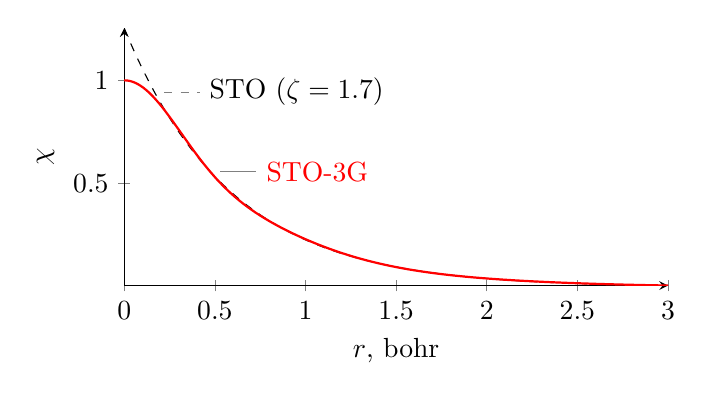
\begin{tikzpicture}[
					      declare function = {
							      gto(\c,\a,\r)=\c*(2*\a/pi)^(3/4)*exp(-\a*\r^2);
							      sto(\z,\r)=sqrt((2*\z)^3/(8*pi))*exp(-\z*\r);
						      },
				      ]
				      \begin{axis}[
						      width=0.7\linewidth,
						      height=0.4\linewidth,
						      axis lines=left,
						      xlabel={$r$, bohr},
						      ylabel=$\chi$,
						      samples=200,
						      domain={0:3},
						      smooth,
					      ]

					      \addplot [dashed]
					      {sto(1.7,x)} node [pos=0.1, pin=0:{STO ($\zeta = 1.7$)}] (s1) {};

					      \addplot [thick, red]
					      {%
						      gto(0.154, 0.636e1, x) +
						      gto(0.535, 0.116e1, x)+
						      gto(0.445, 0.314e0, x)
					      } node [pos=0.2, pin=0:STO-3G] (gs) {};
				      \end{axis}
			      \end{tikzpicture}
		\end{enumerate}
	\end{overlayarea}
\end{frame}

% ============================== Слайд ## ===================================
\begin{frame}{\href{https://en.wikipedia.org/wiki/Slater's_rules}{Способи розрахунку ефективного заряду $\zeta$}}{Правила Слейтера}

	Атоми поділяють на групи
	\[\tcbhighmath[drop fuzzy shadow]{(1s)\quad(2s, 2p)\quad(3s, 3p)\quad(3d)\quad(4s, 4p)\quad(4d)\quad(4f) \ldots} \]
	\begin{overprint}

		\onslide<1>
		\begin{enumerate}
			\item Група електронів, розташована праворуч від розглянутої, вкладу в $\sigma$ не дає;
			\item Кожен електрон в даній групі (крім розглянутого) дає внесок, рівний $0,35$; виняток становлять $1s$-електрони, які дають внесок, рівний $0,30$;
			\item Для $[s,p]$-групи, кожен електрон підоболонки $(n - 1)$ дає внесок, рівний $0,85$, а електрони з підоболонок $(n - 2)$, $(n - 3)$ і т. д. - рівний $1,00$;
			\item Для $[d]$- або $[f]$-груп кожен електрон з подоболонок $(n - 1)$, $(n - 2)$ і т. д. дає внесок, рівний $1,00$.
		\end{enumerate}
		\onslide<2>
		\begin{center}
			Атом Фтора ($(1s^2)\quad (2s^22p^5)$), $Z = 9$)

			\hfill

			\begin{MOdiagram}[style=square]
				\AO{s}[label={1s}]{0;pair}
				\AO{s}[label={2s}]{1;pair}
				\AO(40pt){p}[label={2p}]{1.5;pair,pair,up}
			\end{MOdiagram}
		\end{center}

		Ефективний заряд для $2p$-електрона \(\zeta = 9 - 6\cdot 0.35 - 2\cdot 0.85  = 5.2\) \\
	\end{overprint}
\end{frame}

% ============================== Слайд ## ===================================

\begin{frame}{Ефективний заряд}
	\begin{overprint}
		\onslide<1>
		\begin{figure}
			\centering
			\includegraphics[width=0.5\linewidth]{ZeffWiki}
			\caption{Скріншот \url{https://en.wikipedia.org/wiki/Effective_nuclear_charge}}
			\label{fig:zeffwiki}
		\end{figure}
		\onslide<2>
		\begin{figure}
			\centering
			\includegraphics[width=1\linewidth]{Zeff}
			\caption{\centering Ефективний заряд зовнішніх електронів елементів періодичної таблиці \par
				{\scriptsize  Дані з сайту \url{https://chem.libretexts.org/}}}
			\label{fig:zeff}
		\end{figure}
	\end{overprint}
\end{frame}

% ============================== Слайд ## ===================================
\begin{frame}[t]{Поляризація остова та $n^*$}

		\begin{block}{}\justifying\scriptsize
			Зовнішній електрон діє на остов, поляризуючи його. Поляризація проявляється в відштовхуванні зовнішнім електроном електронів остову, причому чим ближче розташовані електрони тим сильніше вони відштовхуються, тому центральна симетрія порушується і під дією зовнішнього електрона в ядрі наводиться диполь, позитивним кінцем спрямований до електрону. Додаткова взаємодія між електроном і наведеним диполем носить характер притягування і знижує енергію. Це зниження можна врахувати, поправкою до головного квантового числа \[n^* = n + a,\] де $n^*$~--- ефективне квантове число, $a$~--- негативна добавка, яка виникає внаслідок поляризації остова.

			\bigskip

			Поляризовність пропорційна радіусу остова \[\alpha = a_0^3\]
		\end{block}
		По Слейтеру, $n^*$ визначається згідно наступної таблиці:
		\begin{center}
\begin{tblr}{ccccccc}
			\hline
			$n$   & 1   & 2   & 3   & 4   & 5   & 6   \\ \hline
			$n^*$ & 1.0 & 2.0 & 3.0 & 3.7 & 4.0 & 4.2 \\ \hline
		\end{tblr}
\end{center}
\end{frame}

% ============================== Слайд ## ===================================
\begin{frame}[t]{Принципи заповнення атомних орбіталей}
	\begin{overlayarea}{\textwidth}{\textheight}
		\begin{enumerate}
			\item<1-> Принцип Паулі

			      \only<1,4>{
				      \begin{alertblock}{}\justifying
					      Два і більше електрона не можуть одночасно перебувати в одному і тому ж квантовому стані.
				      \end{alertblock}
			      }
			      \only<1>{
				      \begin{center}
					      \includegraphics[width=0.3\linewidth]{PauliPrinciple}
				      \end{center}
			      }
			\item<2-> Правило Маделунга-Клечковського

			      \only<2,4>{
				      \begin{alertblock}{}\justifying
					      Заповнення електронами орбіталей відбувається в порядку зростання суми головного та орбітального квантових чисел $n + l$. При однаковій сумі заповнюється орбіталь з меншим значенням $n$.
				      \end{alertblock}
			      }
			      \only<2>{
				      \begin{center}
					      \includegraphics[width=0.32\linewidth]{RuleFilling}
					      \includegraphics[width=0.22\linewidth]{EnergyLevels}
				      \end{center}
			      }
			\item<3-> Правило Хунда



			      \only<3,4>{
				      \begin{alertblock}{}\justifying
					      Атомні орбіталі, які належать до одного підрівня, заповнюються спочатку електронами з однаковим спіновим числом, а потім електронами з протилежним спіновим числом.
				      \end{alertblock}
			      }
			      \only<3>{
				      \begin{center}
					      \includegraphics[width=0.5\linewidth]{HundsRule}
				      \end{center}
			      }
		\end{enumerate}
	\end{overlayarea}
\end{frame}

%===============================================================================
\begin{frame}{Електронні структури деяких атомів 2-го періоду}
	\begin{center}
		\begin{MOdiagram}[style=square]
			\AO{s}[label={1s}]{0;pair}
			\AO{s}[label={2s}]{1;pair}
			\AO(30pt){p}[label={2p}]{1.5;up,,}
			\node[draw, shape=circle, fill=red!50] at (1.8,-0.5) {\ce{B}};
		\end{MOdiagram}
		\hfill
		\begin{MOdiagram}[style=square]
			\AO{s}[label={1s}]{0;pair}
			\AO{s}[label={2s}]{1;pair}
			\AO(30pt){p}[label={2p}]{1.5;up,up,}
			\node[draw, shape=circle, fill=red!50] at (1.8,-0.5) {\ce{C}};
		\end{MOdiagram}
		\hfill
		\begin{MOdiagram}[style=square]
			\AO{s}[label={1s}]{0;pair}
			\AO{s}[label={2s}]{1;pair}
			\AO(30pt){p}[label={2p}]{1.5;up,up,up}
			\node[draw, shape=circle, fill=red!50] at (1.8,-0.5) {\ce{N}};
		\end{MOdiagram}
		\vfill
		\begin{MOdiagram}[style=square]
			\AO{s}[label={1s}]{0;pair}
			\AO{s}[label={2s}]{1;pair}
			\AO(30pt){p}[label={2p}]{1.5;pair,up,up}
			\node[draw, shape=circle, fill=red!50] at (1.8,-0.5) {\ce{O}};
		\end{MOdiagram}
		\hfill
		\begin{MOdiagram}[style=square]
			\AO{s}[label={1s}]{0;pair}
			\AO{s}[label={2s}]{1;pair}
			\AO(30pt){p}[label={2p}]{1.5;pair,pair,up}
			\node[draw, shape=circle, fill=red!50] at (1.8,-0.5) {\ce{F}};
		\end{MOdiagram}
		\hfill
		\begin{MOdiagram}[style=square]
			\AO{s}[label={1s}]{0;pair}
			\AO{s}[label={2s}]{1;pair}
			\AO(30pt){p}[label={2p}]{1.5;pair,pair,pair}
			\node[draw, shape=circle, fill=red!50] at (1.8,-0.5) {\ce{Ne}};
		\end{MOdiagram}
	\end{center}
\end{frame}

%===============================================================================

\begin{frame}{Електронні структури sp-гібридизованих атомів}
	\begin{center}
		\begin{MOdiagram}[style=square]
			\AO{s}[label={1s}]{0;pair}
			\AO{s}[label={2s}]{1;pair}
			\AO(30pt){p}[label={2p}]{1.5;up,,}
			\node[draw, shape=circle, fill=red!50] at (1.8,-0.5) {\ce{B} (I)};
		\end{MOdiagram}
		\quad
		\begin{MOdiagram}[style=square]
			\AO{s}[label={1s}]{0;pair}
			\AO{s}[label={2s}]{1.5;up}
			\AO(30pt){p}[label={2p}]{1.5;up,up,}
			\node[draw, shape=circle, fill=red!50] at (1.8,-0.3) {\ce{B^*} (III)};
		\end{MOdiagram}
		\vfill
		\begin{MOdiagram}[style=square]
			\AO{s}[label={1s}]{0;pair}
			\AO{s}[label={2s}]{1;pair}
			\AO(30pt){p}[label={2p}]{1.5;up,up,}
			\node[draw, shape=circle, fill=red!50] at (1.8,-0.5) {\ce{C} (II)};
		\end{MOdiagram}
		\quad
		\begin{MOdiagram}[style=square]
			\AO{s}[label={1s}]{0;pair}
			\AO{s}[label={2s}]{1.5;up}
			\AO(30pt){p}[label={2p}]{1.5;up,up,up}
			\node[draw, shape=circle, fill=red!50] at (1.8,-0.3) {\ce{C^*} (IV)};
		\end{MOdiagram}
	\end{center}
\end{frame}

%===============================================================================
\begin{frame}[t]{Розрахунки електронної густини методом Хартрі}
	\begin{overlayarea}{\textwidth}{\textheight}
		Методом самоузгодженого поля можна розрахувати розподіл густини заряду в атомі.
		\only<1>{
			\begin{figure}
				\centering
				\includegraphics[width=1\linewidth]{Ar_Hartree-Fock}
				\caption{З книги <<Quantum Chemistry>> Ira N. Levine, 7ed., Pearson}
				\label{fig:arhartree-fock}
			\end{figure}
		}
		\only<2>{
			\begin{center}
				\includegraphics[width=0.55\linewidth]{AtomicShells}
			\end{center}

			На графіках радіальної густини можна розрізнити $K$-,
			$L$- і $M$-оболонки інертних газів.}
	\end{overlayarea}
\end{frame}

% ===========================================================================



\begin{frame}{Середні радіуси елементів  та іонів }
	\begin{columns}[c]
		\column{.5\textwidth} % column designated by a command
		Середній радіус одноелектронної орбіталі:
		\begin{equation*}
			\tcbhighmath[drop fuzzy shadow]{\left\langle r \right\rangle \approx a_0 \frac32 \frac{n^{*2}}{\zeta}}
		\end{equation*}
		\begin{overprint}
			\onslide<1>
			Середні радіуси елементів.

			{\scriptsize Дані з сайту \url{http://www.basicknowledge101.com}}


			\onslide<2>
			Середні радіуси деяких іонів.

			{\scriptsize Дані з сайту \url{http://www.basicknowledge101.com}}
		\end{overprint}
		\
		\column{.5\textwidth} % column designated by a command
		\begin{overprint}
			\onslide<1>
			\begin{figure}
				\includegraphics[width=0.9\linewidth]{atomicradius}
			\end{figure}
			\onslide<2>
			\begin{figure}
				\includegraphics[width=1\linewidth]{Radii}
			\end{figure}

		\end{overprint}

	\end{columns}
\end{frame}

\begin{frame}{Закон Мозлі}
	Параметри $\zeta$ і $n^*$ були підібрані таким чином, щоб результати оцінок розумно узгоджувалися з експериментальними даними по
	рентгенівським спектрами атомів (закон Мозлі):
	\begin{equation*}\tcbhighmath[drop fuzzy shadow]{
			\nu = \frac{Ry}{2\pi\hbar}\left( \frac{(Z-\sigma_n)^2}{n^2} - \frac{(Z-\sigma_m)^2}{m^2}\right)
		}
	\end{equation*}

	Такі розрахунки були виконані практично для всіх елементів.
\end{frame}

\begin{frame}{Визначення енергії електрона в атомі}

	\begin{equation*}\label{zeta}
		\zeta = \frac{\zeta}{n^*}
	\end{equation*}

	Енергія електрона $\Rightarrow$ як енергія воднеподібного атому:
	\begin{equation*}\label{Energy}
		\tcbhighmath[drop fuzzy shadow]{ \varepsilon = - \frac12\left( \frac{\zeta}{n^*}\right)^2  = -\frac12\zeta^2,}
	\end{equation*}
\end{frame}

\begin{frame}{Енергія іонізації}
	Енергія іонізації --- енергія, необхідна для видалення валентного електрона від вільного атома в його нижчому енергетичному (основному) стані на нескінченність.
	\begin{figure}
		\centering
		\includegraphics[width=0.9\linewidth]{IonizEnergy}
		\caption[Енергія іонізації]{Енергія іонізації}
		\label{fig:ionizenergy}
	\end{figure}
\end{frame}

\begin{frame}{Спорідненість до електрона}
	Спорідненість до електрона~--- енергія, необхідна для того, щоб забрати електрон у однократно від'ємно зарядженого іона.

	Така ж енергія виділяється при захопленні електрона нейтральним атомом чи молекулою.

	\begin{figure}
		\includegraphics[width=1\linewidth]{Electron_affinities_of_the_elements}
		\label{fig:electronaffinitiesoftheelements}
	\end{figure}

\end{frame}


\begin{frame}{Зміна характеристик елементів}
	\begin{figure}
		\centering
		\includegraphics[width=1\linewidth]{SummaryPeriodic}
		\label{fig:summaryperiodic}
	\end{figure}
\end{frame}


\end{document}
